\chapter{Event Reconstruction}\label{chapter:event_reconstruction}

After physics interactions are detected inside of \gls{ATLAS}, are accepted by the trigger system, and are read out to disk they exist as raw detector level information and need to be reconstructed into detector-based representations of physical particles (physics objects) for analysis.
Low latency versions of reconstruction are done at the trigger level to make acceptance decisions.
However, the full event reconstruction is done ``offline'' later with more current detector models and with computationally expensive algorithms with the luxury of time to trade for great accuracy.
This also allows for reprocessing of data in the future with improved algorithms and models.
This chapter gives a high level overview of the physics objects that ATLAS defines and the methods used to make them.
\TODO{Add supporting figures for this chapter during expansion revision.}

\section{Tracks}\label{section:tracks}

One of the most common physics objects is charged tracks, as seen in \Cref{fig:track_cartoon}, representing charged particles passing through the subsystems of the \gls{inner detector}, as discussed in \Cref{sec:ATLAS_ID}, and \gls{muon spectrometer}.
These tracks are reconstructed from hits in these subsystems by using the hit coordinates as inputs to fitting algorithms that generally apply $\chi^{2}$ fitting techniques and Kalman filters to find the track that has the highest likelihood for the observed hits~\cite{Fruhwirth:1987fm,Fruhwirth:2003702,Strandlie:1999,Bugge:1981,Salzburger:2008cea}.

\begin{figure}[htbp]
 \centering
 \includegraphics[width=0.8\linewidth]{event_reconstruction/track_cartoon.png}
 \caption[Cartoon of comparison of the ideal charged track to a possible reconstructed charged track.]{%
  Cartoon of comparison of the ideal charged track (\textcolor{black}{black}) in ATLAS from four hits in the pixel layers and four hits in the strip detectors to a possible reconstructed charged track (\textcolor{red}{red}) that accounts for all of the hits except for one hit in the pixel detector~\cite{Salzburger:HammersAndNails}.}
 \label{fig:track_cartoon}
\end{figure}

\section{Electrons and Photons}\label{section:e_gamma}

Reconstruction of electrons begins with the signals arriving from the ECAL cells after they have been reshaped and sampled~\cite{PERF-2013-05}.
These cells are then converted to energy deposit clusters using hardware calibrations, where the ECAL is divided into a grid of towers of size $\Delta \eta \times \Delta \phi = 0.075 \times 0.175$ in the barrel and $\Delta \eta \times \Delta \phi = 0.125 \times 0.125$ in the end-caps to perform sliding-window scans~\cite{Lampl:1099735} to find local maxima to use as seeds for these clusters~\cite{PERF-2013-05}.
Well-reconstructed tracks from the \gls{inner detector} are then matched to the calorimeter clusters.
The matching of tracks is used to infer if the cluster deposits are from prompt%
\footnote{Prompt decays are where a particle originates from the primary interaction.
Prompt decays are distinguished from non-prompt by their decay time.
An example of a prompt electron would be those originating from $Z\to e^{+}e^{-}$, while a non-prompt electron would be an electron that originated from photon conversion from a radiated photon.}
electrons, electrons from photon conversion, or an unconverted photon~\cite{PERF-2013-05,PERF-2016-01}.
If there is no ID track matched to the cluster, the cluster is selected as an unconverted photon.
The fine granularity in $\eta$ of the silicon strip detectors is sufficient to provide event-by-event discrimination between single-photon showers and two overlapping showers originating from the decays of neutral hadrons (mostly $\pi^{0}$ and $\eta$ mesons) in the fiducial region $\abs{\eta} < 1.37$ and $1.52 < \abs{\eta} < 2.37$~\cite{PERF-2017-02}.
If the cluster is matched to a pair of oppositely charged ID tracks that are collinear from the primary vertex and additionally have signatures in the TRT that are consistent with electrons then the clusters are identified as a converted photon.
In all other cases where there are matched ID tracks to calorimeter clusters, the clusters are identified as electrons.

In addition, electrons candidates have additional quality and isolation identification performed.
There are three levels of electron quality ``working points'': \texttt{Loose}, \texttt{Medium}, and \texttt{Tight}.
These working points are effectively minimum values of a multivariate likelihood ratio based discriminate which an analyst can then ``cut'' on to make acceptance decisions.
Isolation criteria are determined using a track-based isolation variable, $p_{T}^{\mathrm{varcone30}}$, and a calorimeter-based isolation variable, $E_{T}^{\mathrm{topcone20}}$.
The isolation criteria compare the scalar sum of the transverse momentum in a cone around the electron candidate track of size $\Delta R < 0.2$ for $E_{T}^{\mathrm{topcone20}}$ and $\Delta R < 0.3$ for $p_{T}^{\mathrm{varcone30}}$ and the transverse momentum of the electron candidate.
This provides an effective discriminant between prompt electron candidates and other electron candidates.

Electrons are also calibrated to data using the well known and characterized resonant decays of $J/\Psi \to e^{+}e^{-}$, $Z \to e^{+}e^{-}$, and $Z \to \ell^{+}\ell^{-}\gamma$.
This calibration is done to derive data-driven scale factors that can be applied to ensure uniformity in the detector response across different subsystems and regions and to establish systematic uncertainties that can cover discrepancies between simulation and data.

\section{Muons}\label{section:muons}

Reconstruction of muons uses tracks from both the \gls{inner detector} and the \gls{muon spectrometer}~\cite{PERF-2015-10}.
The tracks from the ID are reconstructed in the same manner as other charged particles, and the reconstruction algorithms in the MS look for hit patterns in each muon chamber to create unique chamber track segments.
Four muon candidate types are defined based on the combination of subdetectors used in the reconstruction.
Combined (CB) muons are constructed from combined, global refits of the ID and MS tracks by adding or removing tracks from the MS to improve the quality of the fit.
Segment-tagged (ST) muons are constructed by identifying tracks in the ID as muon tracks if there is an associated track to it in the \gls{MDT} or \gls{CSC}.
ST muon candidates are primarily low $p_{T}$ muons that do not traverse the entire MS.
Calorimeter-tagged (CT) muons are constructed from ID tracks and an ECAL deposit consistent with a minimum ionizing particle.
Extrapolated (ME) muons are constructed from MS tracks in at least two layers that point back to the primary vertex.
ME muon candidates are used to extend the acceptance of muon reconstruction outside the ID in the region of $2.5 < \abs{\eta} < 2.7$ where there is no ID coverage.
With regards to priority when there is overlap of muons of various categories, more information is preferred and so the (decreasing) priority ordering is CB, ST, CT.
If there is overlap with ME muons additional track quality information is required to resolve priority.

Like electrons, muon quality working points are established, and four are used in ATLAS.
For the \texttt{loose} working point all muon types are used.
This is useful for analyses where it is beneficial to maximize reconstruction efficiency above other concerns, such as $H \to 4\ell$.
The \texttt{medium} working point CB and ME tracks are used where there are at least three CB track hits and three ME layers.
The \texttt{tight} working point is designed to maximize muon purity and only used CB muons which have hits in at least two layers of the MS and also satisfy the \texttt{medium} working point requirements.
Finally, the high-$p_{T}$ working point requires CB muons passing the \texttt{medium} selection with at least three hits in the MS.
This working point is designed to maximize the momentum resolution for muon tracks with $p_{T} > 100~\GeV$.
Additionally, there are muon isolation requirements.
These isolation requirements use the track-based isolation variable, $p_{T}^{\mathrm{varcone30}}$, and a calorimeter-based isolation variable, $E_{T}^{\mathrm{topcone20}}$, described in \Cref{section:e_gamma}.
Muons are also further calibrated to data using $J/\Psi \to \mu^{+}\mu^{-}$ to cover the low $p_{T}$ spectrum and $Z \to \mu^{+}\mu^{-}$ for the high $p_{T}$ spectrum, as shown in \Cref{fig:dimuon_efficiency_scale_factor_uncert}.

\begin{figure}[htbp]
 \centering
 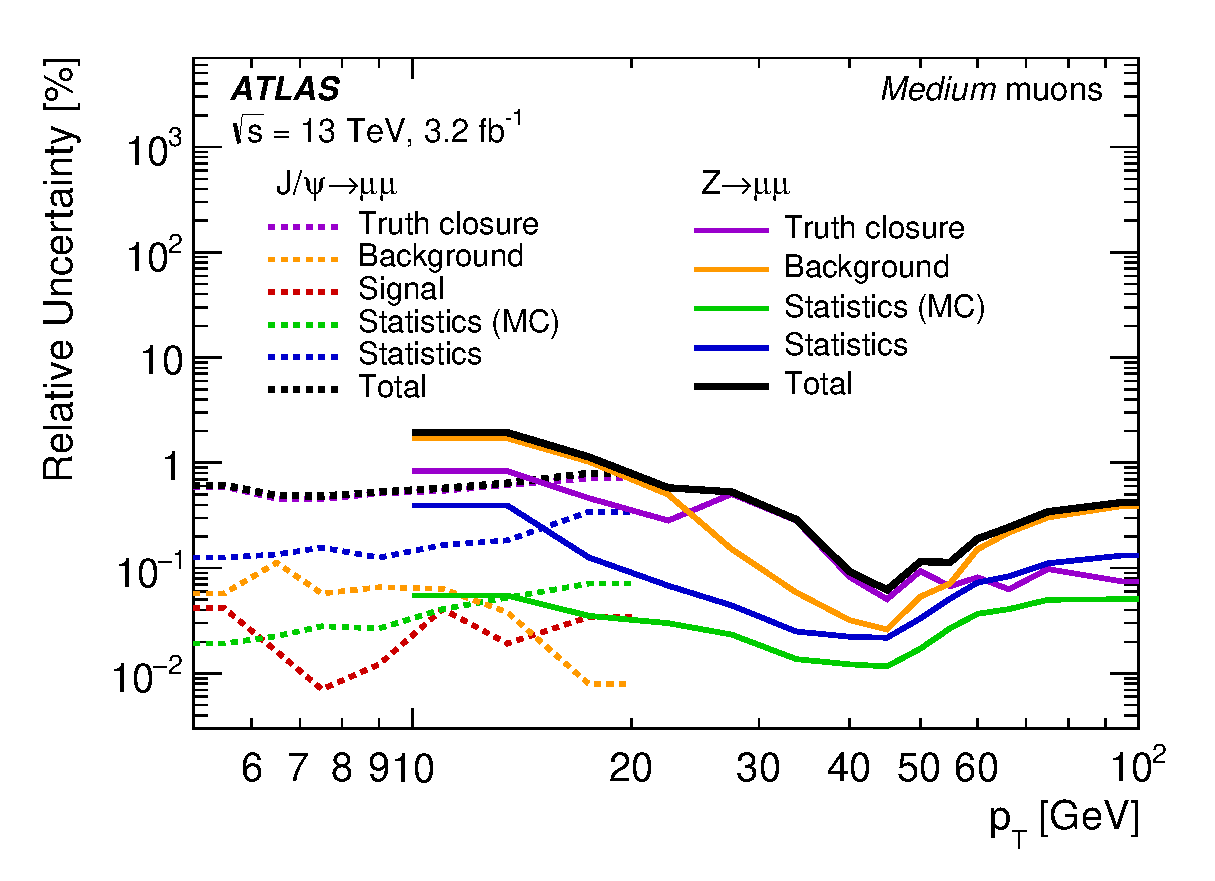
\includegraphics[width=0.8\linewidth]{event_reconstruction/dimuon_efficiency_scale_factor_uncert.eps}
 \caption[Total uncertainty in the efficiency scale factor for Medium muons as a function of $p_{T}$ as obtained from $Z\to\mu\mu$ and $J/\Psi \to \mu\mu$ decays.]{%
  Total uncertainty in the efficiency scale factor for Medium muons as a function of $p_{T}$ as obtained from $Z\to\mu\mu$ (solid lines) and $J/\Psi \to \mu\mu$ (dashed lines) decays.
  The combined uncertainty is the sum in quadrature of the individual contributions~\cite{PERF-2015-10}.}
 \label{fig:dimuon_efficiency_scale_factor_uncert}
\end{figure}

\section{Jets}\label{section:jets}

As particles that carry \gls{QCD} color charge do not exist by themselves in isolation, but form with other colored particles to form colorless composite particles known as ``hadrons,'' it is not possible to directly observe quarks or gluons in ATLAS.
Instead, this process of hadronization, and subsequent decays and rehadronization, creates a shower of both charged and neutral particles that hit the detector, creating charged tracks and energy deposits.
These hadronic showers are stochastic, and there is no way to give a full descriptive definition of them, though there is very impressive recent work on operational definitions~\cite{Metodiev:2018ftz,Komiske:2018vkc,Larkoski:2019nwj}.
Instead, clustering algorithms are used to create collections of tracks and energy deposits, known as ``jets'', based off of the criteria of interest in the algorithm.
In a similar manner to how QCD's depth and richness as a theory requires proper treatment outside the scope of this thesis, jet physics is complex and deep enough to rightly be its own intense physics program at the LHC.
This section will only attempt to give an executive summary of the jet physics and techniques that is pertinent to my thesis analysis --- however for an exceedingly thorough overview see~\cite{Nachman:2016qyc}.

Of the jet clustering algorithms that are common in high energy physics~\cite{Salam:2009jx,Salam:2007xv} the most widely used are the $k_{t}$, Cambridge/Aachen, and anti-$k_{t}$ algorithms~\cite{Cacciari:2008gp,Soyez:2008pq}.
These algorithms are all similar in their approaches with variations on the features they emphasize.
The approach is to iteratively apply the following for all objects in the considered RoI:
\begin{enumerate}
 \item Compute the pairwise distance $d_{ij}$ between objects $i$ and $j$ where
       \[
        d_{ij} = \textrm{min}\left(k_{ti}^{2p}, k_{tj}^{2p}\right) \frac{\Delta_{ij}^{2}}{R^{2}}
       \]
       and $\Delta_{ij}^{2} = \left(y_{i} - y_{j}\right)^{2} + \left(\phi_{i} - \phi_{j}\right)^{2}$ for transverse momentum $k_{t}$, rapidity $y$, and azimuthal angle $\phi$, and parameters of choice $R$, which governs the size of the jet (though it is not a hard cutoff limit), and $p$, which governs the relative power of the energy versus geometrical $\left(\Delta_{ij}\right)$ scales~\cite{Cacciari:2008gp}.
 \item Compute the distance $d_{iB}$ between the object $i$ and the beamline $B$ where $d_{iB} = k_{ti}^{2p}$.
 \item Determine the smallest distance out of the set of distances $d_{ij}$ and $d_{iB}$, $d_{\mathrm{min}} \in \left\{\left\{d_{ij}\right\},\left\{d_{iB}\right\}\right\}$.
 \item If the minimum distance is between the object $i$ and the beamline, $d_{\mathrm{min}} \in \left\{d_{iB}\right\}$, label this object a jet and remove it.
 \item If the minimum distance is between object $i$ and $j$, $d_{\mathrm{min}} \in \left\{d_{ij}\right\}$, group these two objects into a new object $k$ which is added to the object collection, and remove objects $i$ and $j$.
\end{enumerate}
The above is repeated until there are no more remaining objects, at which point all objects have been assigned to a jet.
It is seen that the choice of free parameter $p$ then defines which algorithm is used, and what information the jet clustering algorithm prioritizes.
The choice of $p=1$ corresponds to the $k_{t}$ algorithm~\cite{Catani:1993hr}, which is seen to cluster softer --- less energetic --- objects together into progressively harder --- more energetic --- objects, as seen in \Cref{fig:jet_algorithms_kt}.
Working under the assumption that generally the hardest objects will be towards the center of the shower of particles, this can be seen as an ``outside-in'' clustering which will result in irregularly shaped (probably not very cone-like) jets.
Choosing $p=0$ corresponds to the Cambridge/Aachen jet algorithm~\cite{Dokshitzer:1997in}, which reduces the distance $d_{ij}$ to only include the angular information, $\Delta_{ij}$.
This means that softer splittings of the shower will be clustered into harder branches, which will again produce irregular shaped jets, as seen in \Cref{fig:jet_algorithms_Cambridge_Aachen}.
Choosing $p=-1$ corresponds to the anti-$k_{t}$ algorithm~\cite{Cacciari:2008gp}, where the hardest objects are clustered together first and then subsequently softer objects are added.
The anti-$k_{t}$ algorithm produces relatively regular cone shaped jets that are focused around a hard core, as seen in \Cref{fig:jet_algorithms_anti_kt}.
A typical choice of jet algorithm in ATLAS is the anti-$k_{t}$ algorithm with size parameter of $R=0.4$.

\begin{figure}[htbp]
 \centering
 \begin{subfigure}[t]{0.315\textwidth}
  \centering
  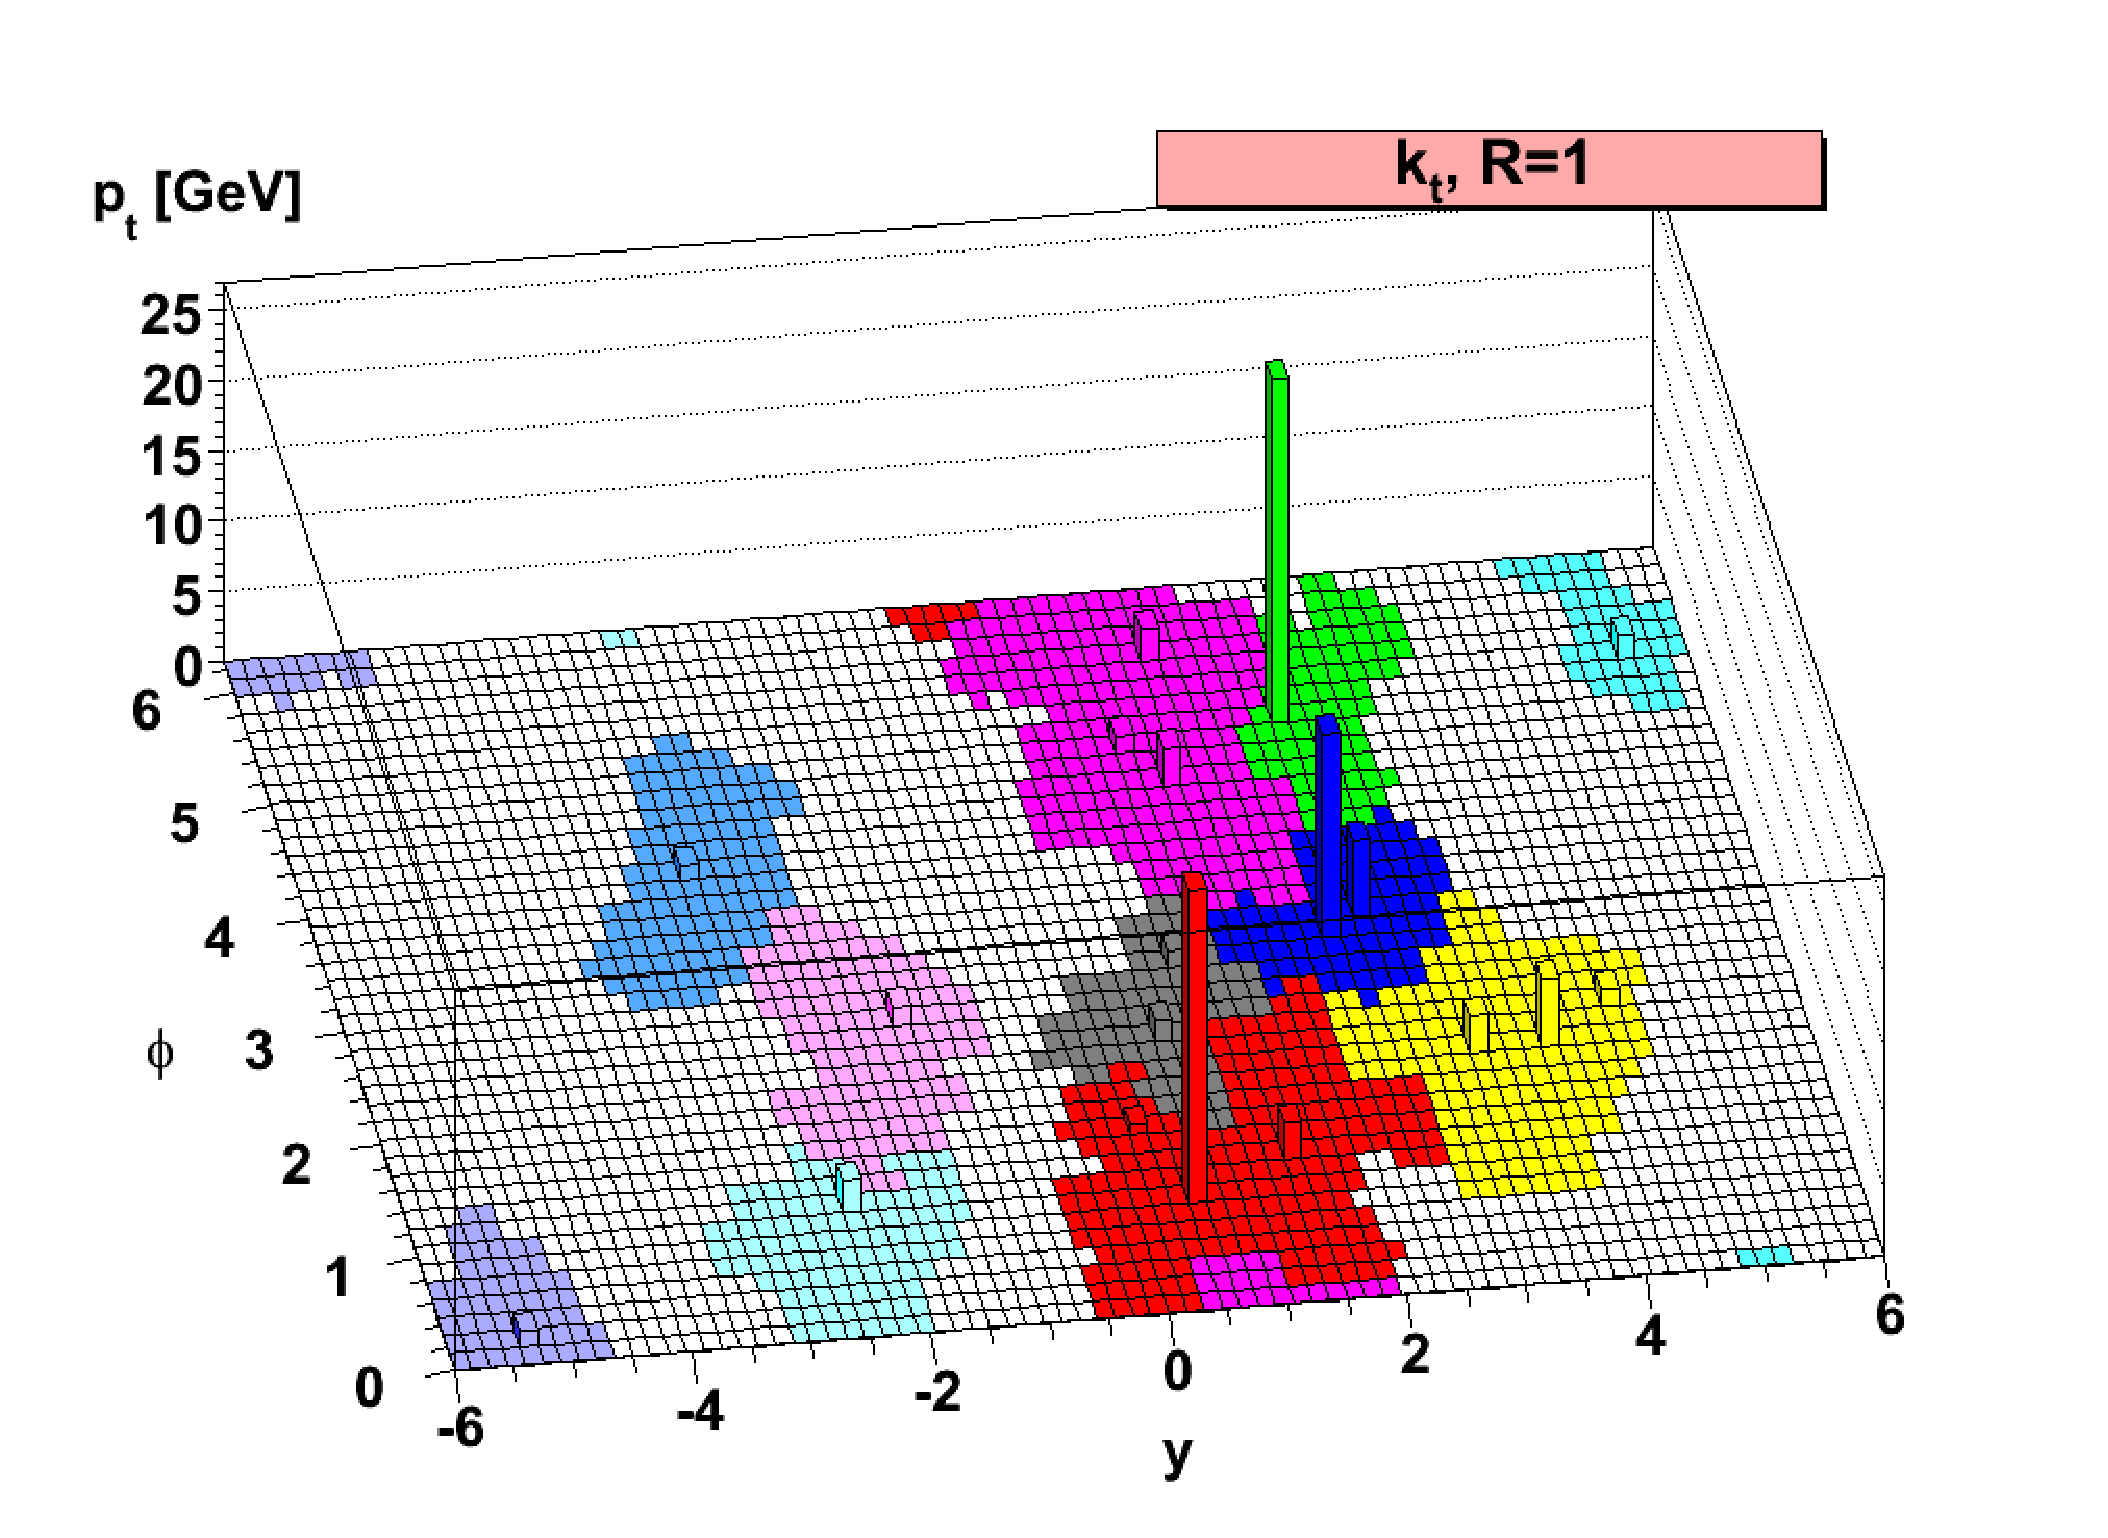
\includegraphics[width=\textwidth]{event_reconstruction/kt.eps}
  \caption[The sample parton-level event clustered with the $k_{t}$ jet algorithm.]{%
   The sample parton-level event clustered with the $k_{t}$ jet algorithm.}
  \label{fig:jet_algorithms_kt}
 \end{subfigure}%
 \quad
 \begin{subfigure}[t]{0.315\textwidth}
  \centering
  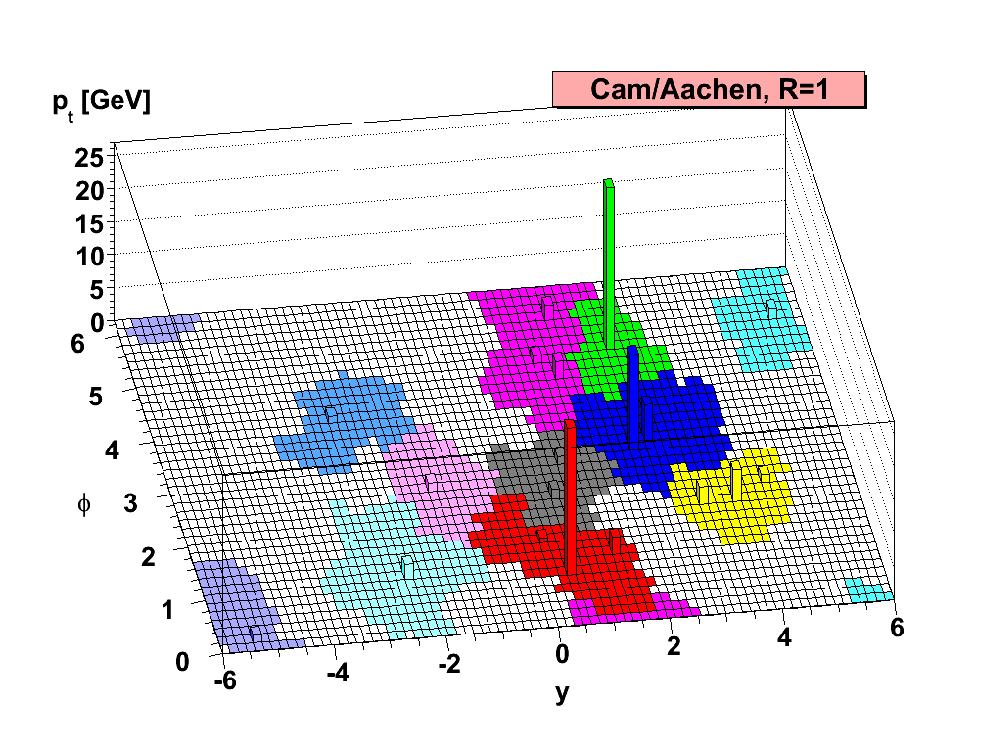
\includegraphics[width=\textwidth]{event_reconstruction/Cambridge_Aachen.eps}
  \caption[The sample parton-level event clustered with the Cambridge/Aachen jet algorithm.]{%
   The sample parton-level event clustered with the Cambridge/Aachen jet algorithm.}
  \label{fig:jet_algorithms_Cambridge_Aachen}
 \end{subfigure}%
 \quad
 \begin{subfigure}[t]{0.315\textwidth}
  \centering
  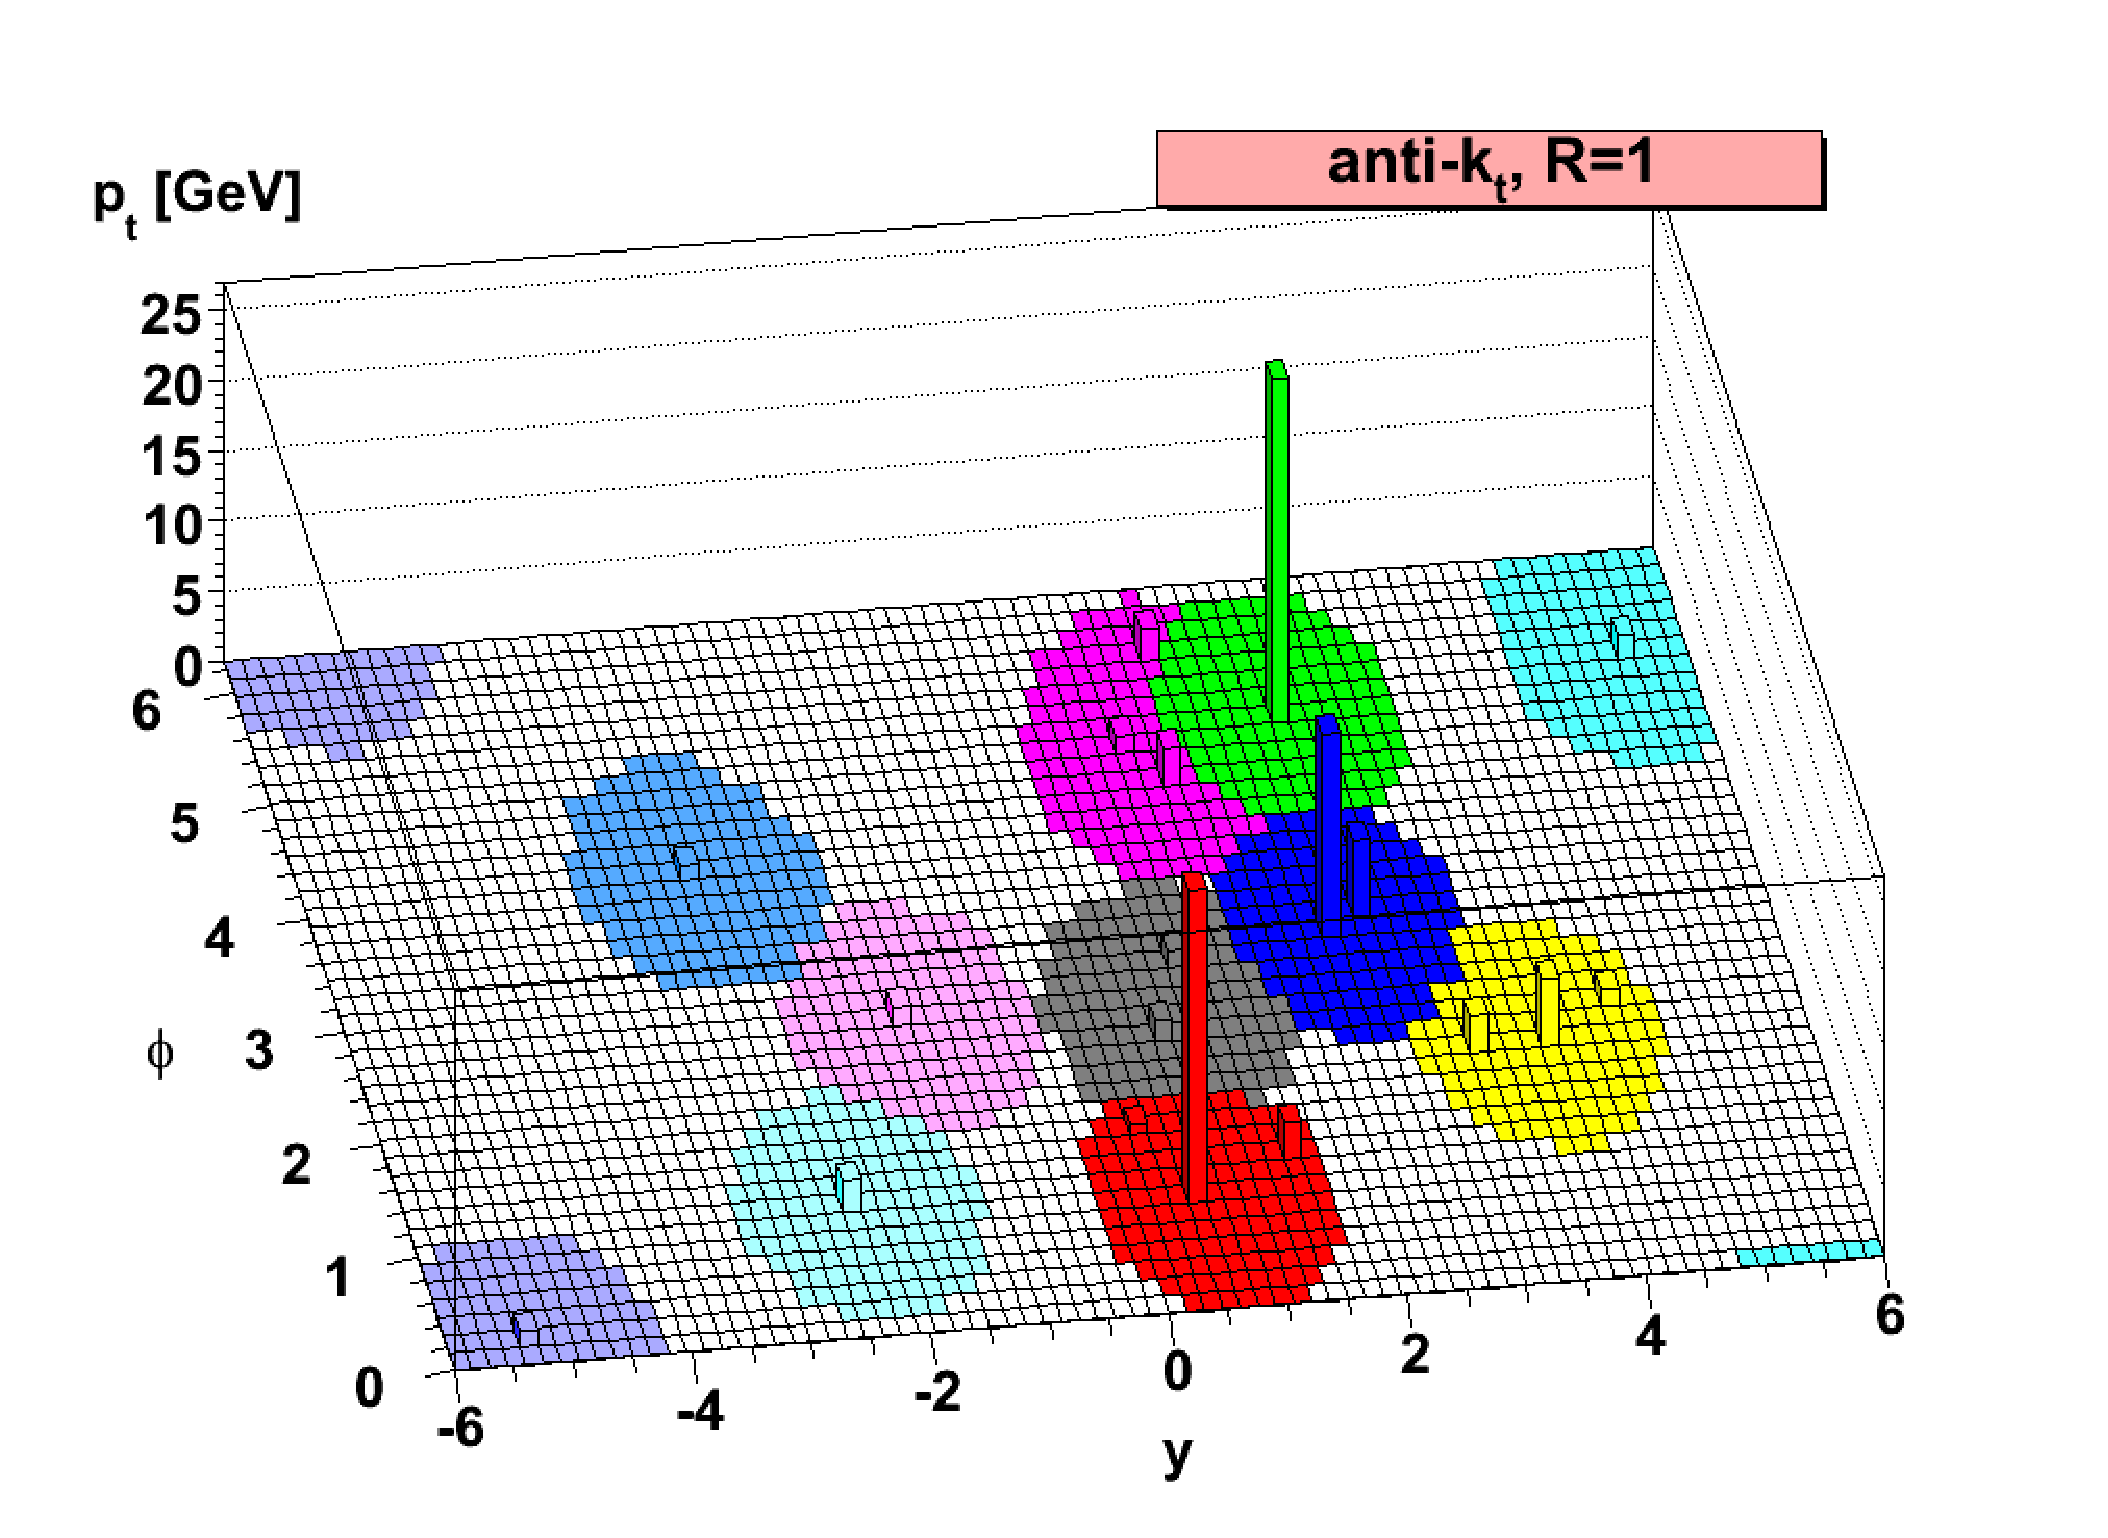
\includegraphics[width=\textwidth]{event_reconstruction/anti_kt.eps}
  \caption[The sample parton-level event clustered with the anti-$k_{t}$ jet algorithm.]{%
   The sample parton-level event clustered with the anti-$k_{t}$ jet algorithm.}
  \label{fig:jet_algorithms_anti_kt}
 \end{subfigure}%
 \caption[A sample parton-level event, together with many random soft ``ghosts'', clustered with three different jet algorithms, illustrating the ``active'' catchment areas of the resulting hard jets.]{%
  A sample parton-level event (generated with Herwig), together with many random soft ``ghosts'', clustered with the $k_{t}$, Cambridge/Aachen, and anti-$k_{t}$ jet algorithms, illustrating the ``active'' catchment areas of the resulting hard jets.
  For $k_{t}$ and Cambridge/Aachen the detailed shapes are in part determined by the specific set of ghosts used, and change when the ghosts are modified~\cite{Cacciari:2008gp}.}
 \label{fig:jet_algorithms}
\end{figure}


\subsection{Large Radius Jets}\label{subsection:largeR_jets}

For analyses that are dealing with very high momentum resonances, the resulting decay products can become highly collimated and be reconstructed as a single jet with a large radius parameter, $R$, (a ``\largeR{}'' jet) typically set to $R=1.0$~\cite{JETM-2018-02,SUSY-2016-13}.
For my thesis analysis \largeR{} jets were used, where the \largeR{} jets were reconstructed from topological clusters in the calorimeters using the anti-$k_{t}$ algorithm with radius parameter of $R=1.0$ and were trimmed~\cite{Krohn:2009th} to improve mass resolution and reduce dependence on pile-up.
The trimming is done by reclustering the \largeR{} jet constituents using the $k_{t}$ algorithm with a radius parameter of $R=0.2$ into subjets, and then removing any subjet that has $p_{T}$ less than $5\%$ of the \largeR{} parent jet's energy.

\subsection{Variable Radius Track Jets}\label{subsection:VR_jets}

In recent years there have been dedicated efforts to improve jet algorithm techniques, especially in the high momentum regime.
As part of these efforts, variable radius (VR) jets~\cite{Krohn:2009zg,ATL-PHYS-PUB-2017-010} were introduced where the radius parameter, $R$, decreases as a function of the jet $p_{T}$,
\[
 R_{\mathrm{eff}} \left(p_{T}\right)= \frac{\rho}{p_{T}},
\]
where the dimensionful constant $\rho$ determines how fast the effective jet size decreases with the transverse momentum of the jet.
The choice of $\rho$ should be proportional to the mass of the resonance, and so should correctly reproduce the size of jets as long as $\rho \lesssim 2 p_{T}$.
Additional parameters $R_{\mathrm{min}}$ and $R_{\mathrm{max}}$ are used to to impose
lower and upper cut-offs on the jet size,
\[
 R_{\mathrm{eff}} \left(p_{T}\right)= \mathrm{max}\left[\mathrm{min}\left(\frac{\rho}{p_{T}},R_{\mathrm{max}}\right),R_{\mathrm{min}}\right]\,.
\]
For my thesis analysis variable radius track jets~\cite{Zenz:2010hfa} were used with $\rho=30~\GeV$, $R_{\mathrm{min}}=0.02$, and $R_{\mathrm{max}}=0.4$, which in simulation gives the highest truth sujbet double $b$-labelling efficiency across for high $p_{T}$ Higgs bosons~\cite{ATL-PHYS-PUB-2017-010}, as seen in \Cref{fig:VR_jets_parameters}.
It is seen from \Cref{fig:VR_jets_lead_subjet}, \Cref{fig:VR_jets_sublead_subjet}, and \Cref{fig:Higgs_VR_DeltaR} that VR track jets are able to describe the topology of $\Hbb$ events across high $p_{T}$ spectrum much more accurately than fixed radius $R=0.2$ track jets, making their use an excellent choice for the analysis.

\begin{figure}[htbp]
 \centering
 \begin{subfigure}[t]{0.48\textwidth}
  \centering
  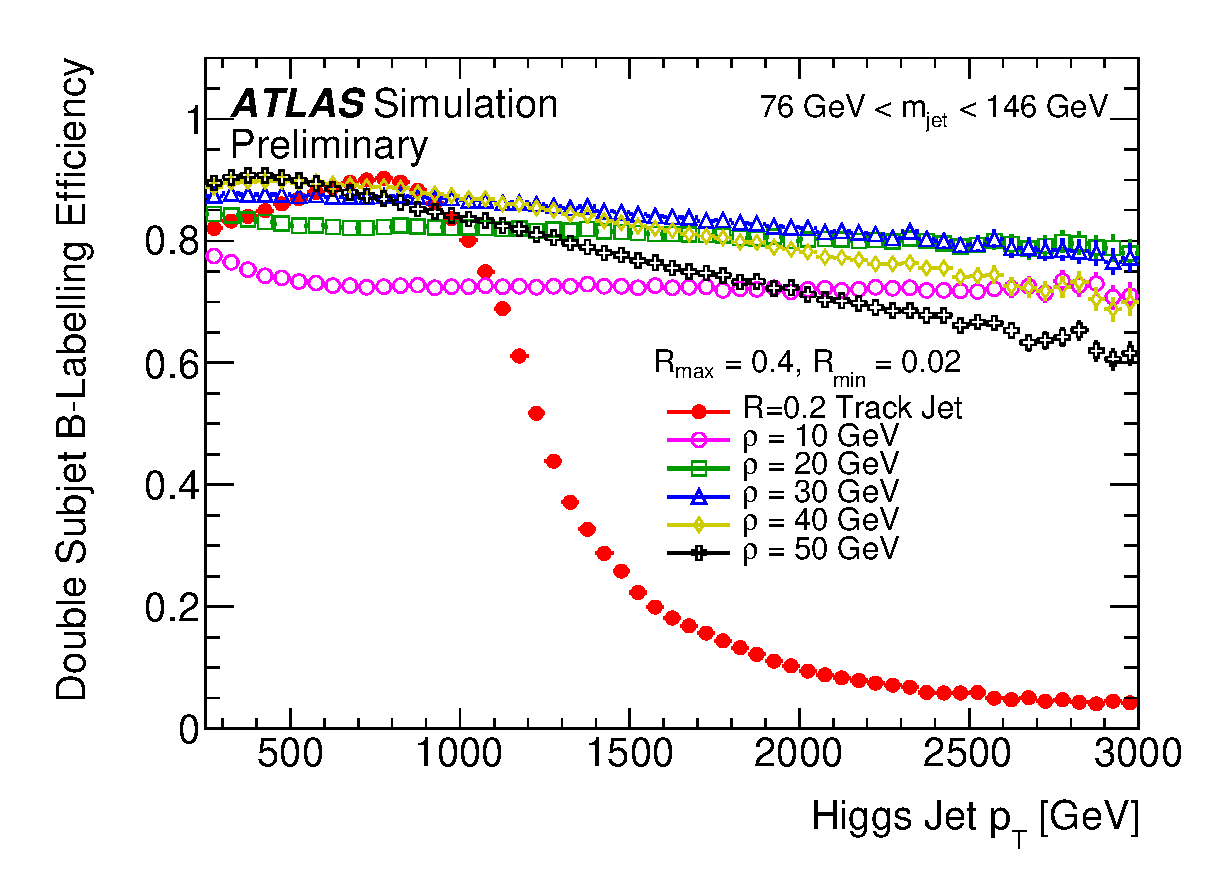
\includegraphics[width=\textwidth]{event_reconstruction/VR_jets_rho_values.eps}
  \caption[The efficiency for VR track jets with ${R_{\mathrm{min}}=0.02}$ and ${R_{\mathrm{max}} = 0.4}$ for several $\rho$ values.]{%
   The efficiency for VR track jets with ${R_{\mathrm{min}}=0.02}$ and ${R_{\mathrm{max}} = 0.4}$ for several $\rho$ values.}
  \label{fig:VR_jets_rho_values}
 \end{subfigure}%
 \quad
 \begin{subfigure}[t]{0.48\textwidth}
  \centering
  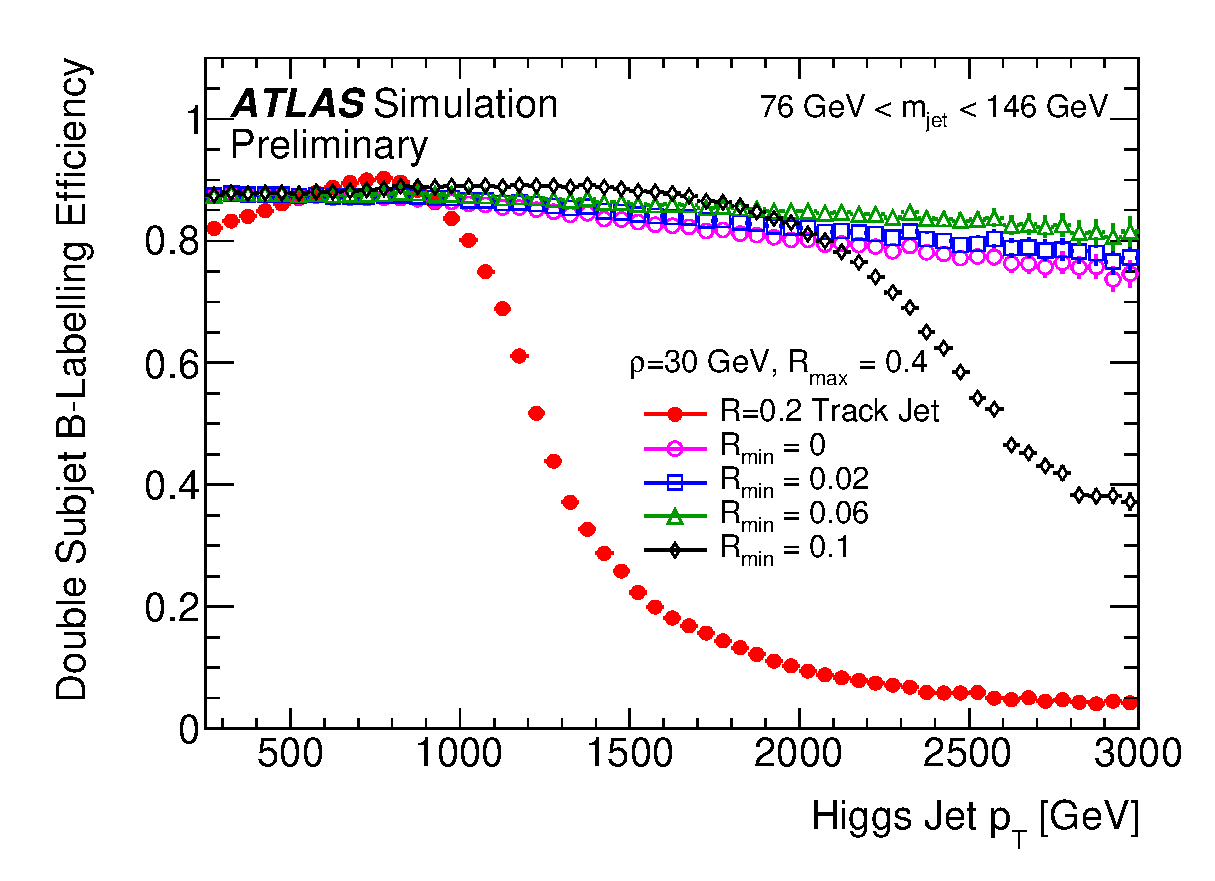
\includegraphics[width=\textwidth]{event_reconstruction/VR_jets_Rmin.eps}
  \caption[The efficiency for VR track jets with ${\rho=30~\GeV}$ and ${R_{\mathrm{max}} = 0.4}$ for different values of $R_{\mathrm{min}}$.]{%
   The efficiency for VR track jets with ${\rho=30~\GeV}$ and ${R_{\mathrm{max}} = 0.4}$ for different values of $R_{\mathrm{min}}$.}
  \label{fig:VR_jets_Rmin}
 \end{subfigure}%

 \begin{subfigure}[t]{0.48\textwidth}
  \centering
  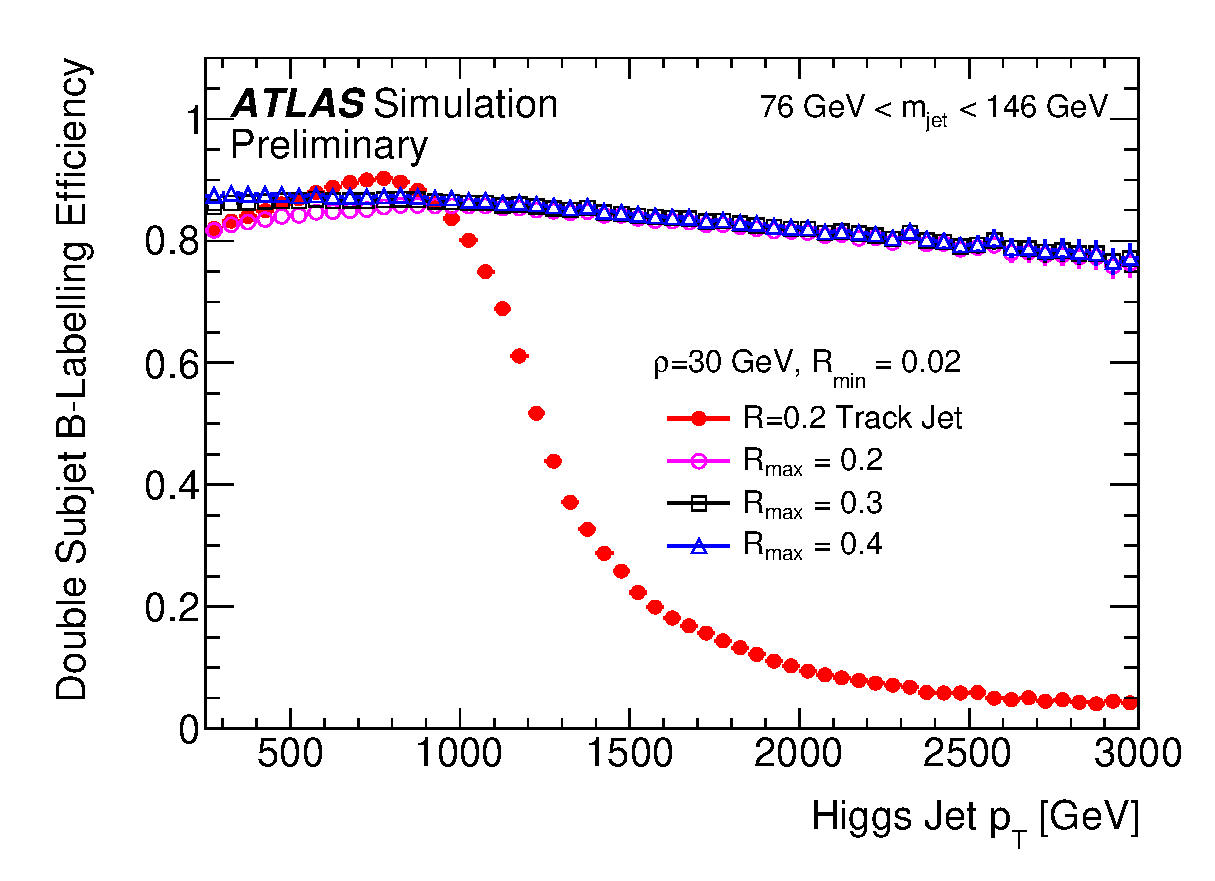
\includegraphics[width=\textwidth]{event_reconstruction/VR_jets_Rmax.eps}
  \caption[The efficiency for VR track jets with ${\rho=30~\GeV}$ and ${R_{\mathrm{min}} = 0.02}$ for varying values of $R_{\mathrm{max}}$.]{%
   The efficiency for VR track jets with ${\rho=30~\GeV}$ and ${R_{\mathrm{min}} = 0.02}$ for varying values of $R_{\mathrm{max}}$.}
  \label{fig:VR_jets_Rmax}
 \end{subfigure}%
 \caption[Efficiency of subjet double $b$-labelling at the truth level of a Higgs jet as a function of the Higgs jet $p_{T}$.]{%
  Efficiency of subjet double $b$-labelling at the truth level of a Higgs jet as a function of the Higgs jet $p_{T}$.
  The efficiency for $R=0.2$ track jets is also included in all of the plots.
  The uncertainty bars include statistical uncertainties only~\cite{ATL-PHYS-PUB-2017-010}.}
 \label{fig:VR_jets_parameters}
\end{figure}

\begin{figure}[htbp]
 \centering
 \begin{subfigure}[t]{0.48\textwidth}
  \centering
  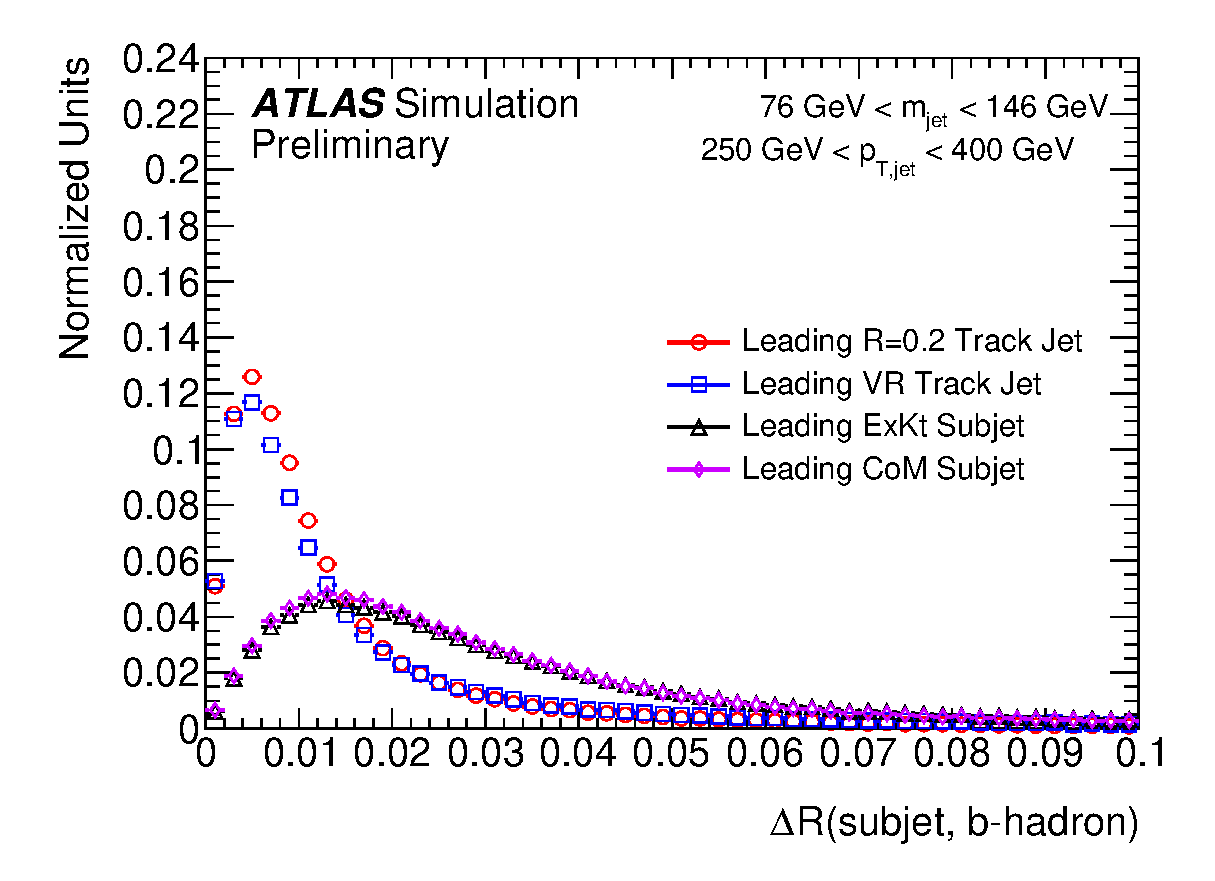
\includegraphics[width=\textwidth]{event_reconstruction/VR_jets_lead_subjet_low.eps}
  \caption[Distributions of the $\Delta R$ between leading subjets and matched truth $b$-hadrons for Higgs with low jet $p_{T}$ of ${250~\GeV < p_{T} < 400~\GeV}$.]{%
   Distributions of the $\Delta R$ between leading subjets and matched truth $b$-hadrons for Higgs with low jet $p_{T}$ of ${250~\GeV < p_{T} < 400~\GeV}$.}
  \label{fig:VR_jets_lead_subjet_low}
 \end{subfigure}%
 \quad
 \begin{subfigure}[t]{0.48\textwidth}
  \centering
  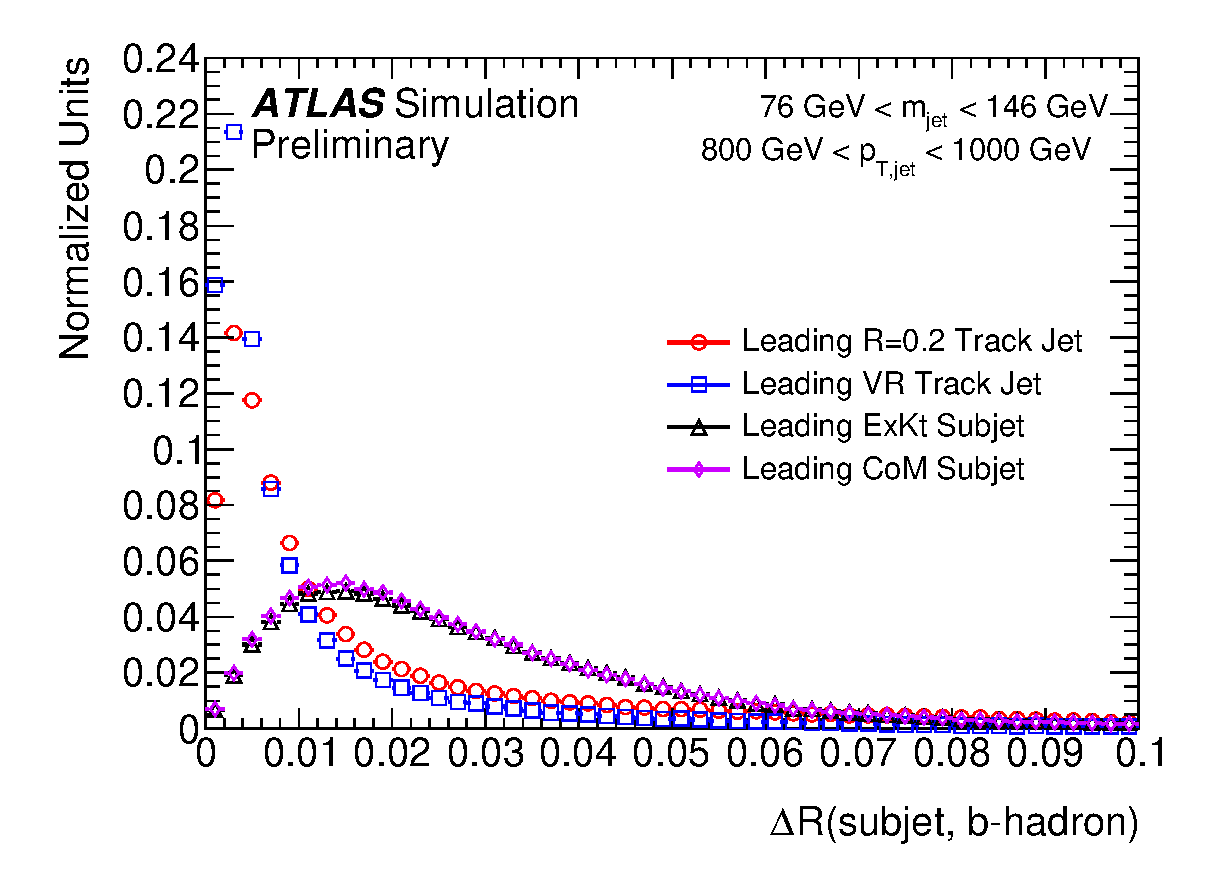
\includegraphics[width=\textwidth]{event_reconstruction/VR_jets_lead_subjet_high.eps}
  \caption[Distributions of the $\Delta R$ between leading subjets and matched truth $b$-hadrons for Higgs with high jet $p_{T}$ of ${800~\GeV < p_{T} < 1000~\GeV}$.]{%
   Distributions of the $\Delta R$ between leading subjets and matched truth $b$-hadrons for Higgs with high jet $p_{T}$ of ${800~\GeV < p_{T} < 1000~\GeV}$.}
  \label{fig:VR_jets_lead_subjet_high}
 \end{subfigure}%
 \caption[Distributions of the $\Delta R$ between leading subjets and matched truth $b$-hadrons for two different Higgs jet $p_{T}$ bins.]{%
  Distributions of the $\Delta R$ between leading subjets and matched truth $b$-hadrons for low Higgs jet $p_{T}$ of ${250~\GeV < p_{T} < 400~\GeV}$ and high Higgs jet $p_{T}$ of ${800~\GeV < p_{T} < 1000~\GeV}$.
  The uncertainty bars include statistical uncertainties only.
  All algorithms have been normalized to an area corresponding to the fraction of signal jets which contain a leading subjet~\cite{ATL-PHYS-PUB-2017-010}.}
 \label{fig:VR_jets_lead_subjet}
\end{figure}

\begin{figure}[htbp]
 \centering
 \begin{subfigure}[t]{0.48\textwidth}
  \centering
  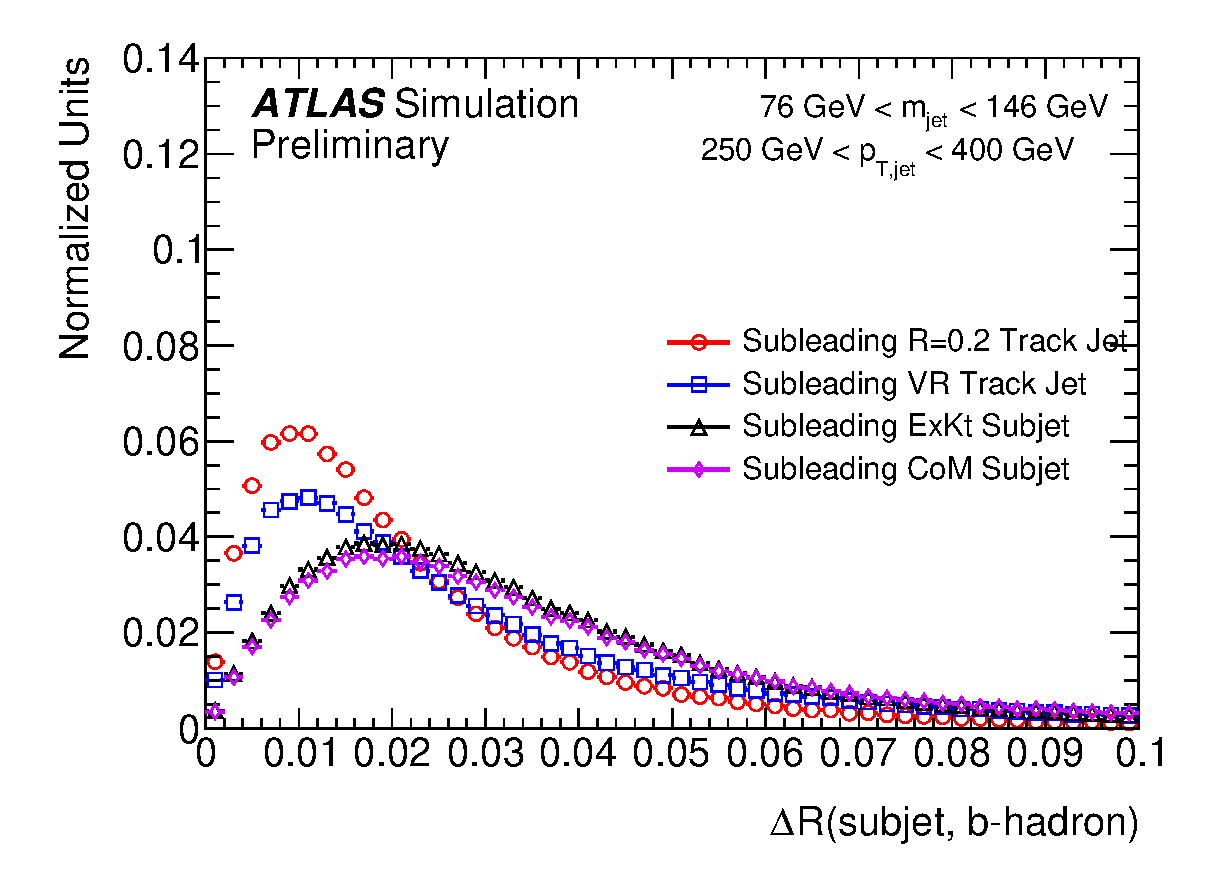
\includegraphics[width=\textwidth]{event_reconstruction/VR_jets_sublead_subjet_low.eps}
  \caption[Distributions of the $\Delta R$ between subleading subjets and matched truth $b$-hadrons for Higgs with low jet $p_{T}$ of ${250~\GeV < p_{T} < 400~\GeV}$.]{%
   Distributions of the $\Delta R$ between subleading subjets and matched truth $b$-hadrons for Higgs with low jet $p_{T}$ of ${250~\GeV < p_{T} < 400~\GeV}$.}
  \label{fig:VR_jets_sublead_subjet_low}
 \end{subfigure}%
 \quad
 \begin{subfigure}[t]{0.48\textwidth}
  \centering
  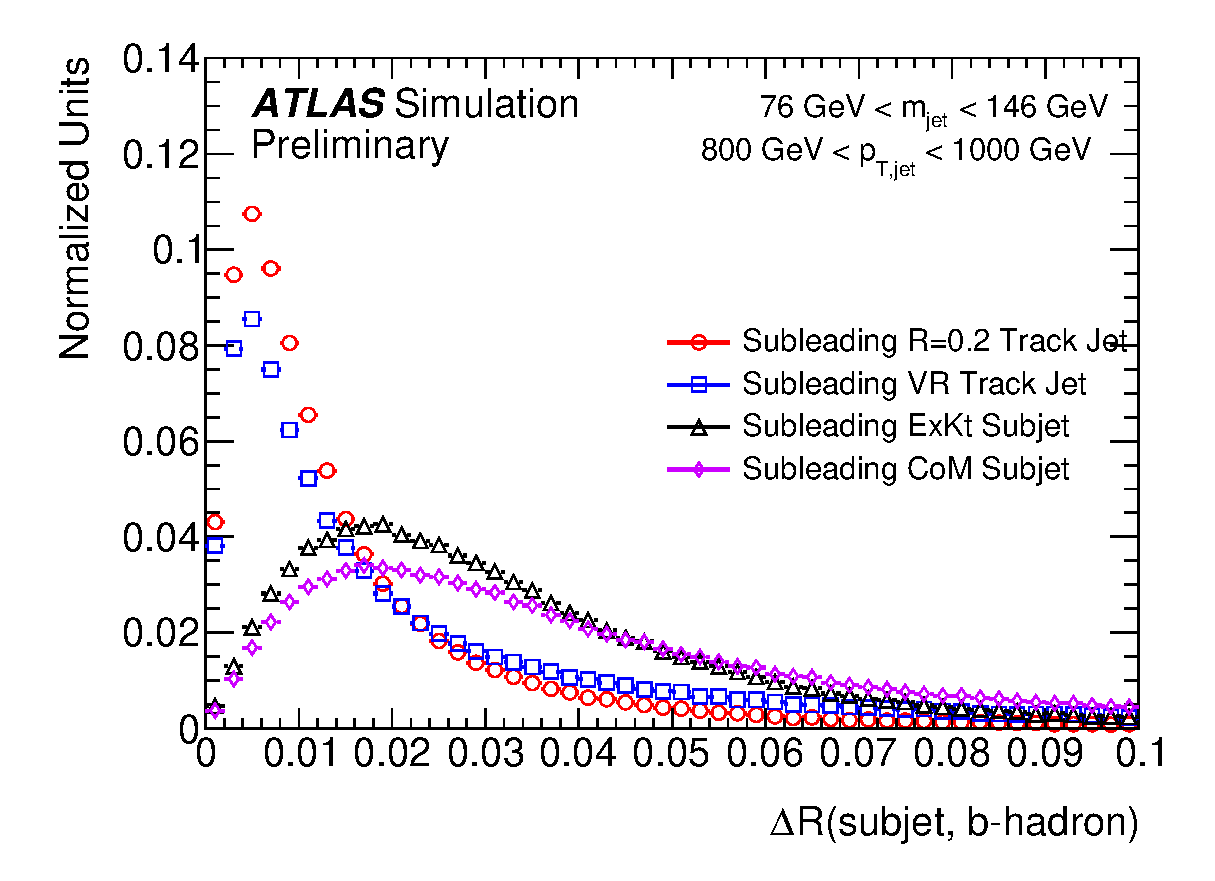
\includegraphics[width=\textwidth]{event_reconstruction/VR_jets_sublead_subjet_high.eps}
  \caption[Distributions of the $\Delta R$ between subleading subjets and matched truth $b$-hadrons for Higgs with high jet $p_{T}$ of ${800~\GeV < p_{T} < 1000~\GeV}$.]{%
   Distributions of the $\Delta R$ between subleading subjets and matched truth $b$-hadrons for Higgs with high jet $p_{T}$ of ${800~\GeV < p_{T} < 1000~\GeV}$.}
  \label{fig:VR_jets_sublead_subjet_high}
 \end{subfigure}%
 \caption[Distributions of the $\Delta R$ between subleading subjets and matched truth $b$-hadrons for two different Higgs jet $p_{T}$ bins.]{%
  Distributions of the $\Delta R$ between subleading subjets and matched truth $b$-hadrons for low Higgs jet $p_{T}$ of ${250~\GeV < p_{T} < 400~\GeV}$ and high Higgs jet $p_{T}$ of ${800~\GeV < p_{T} < 1000~\GeV}$.
  The uncertainty bars include statistical uncertainties only.
  All algorithms have been normalized to an area corresponding to the fraction of signal jets which contain a leading subjet~\cite{ATL-PHYS-PUB-2017-010}.}
 \label{fig:VR_jets_sublead_subjet}
\end{figure}

\begin{figure}[htbp]
 \centering
 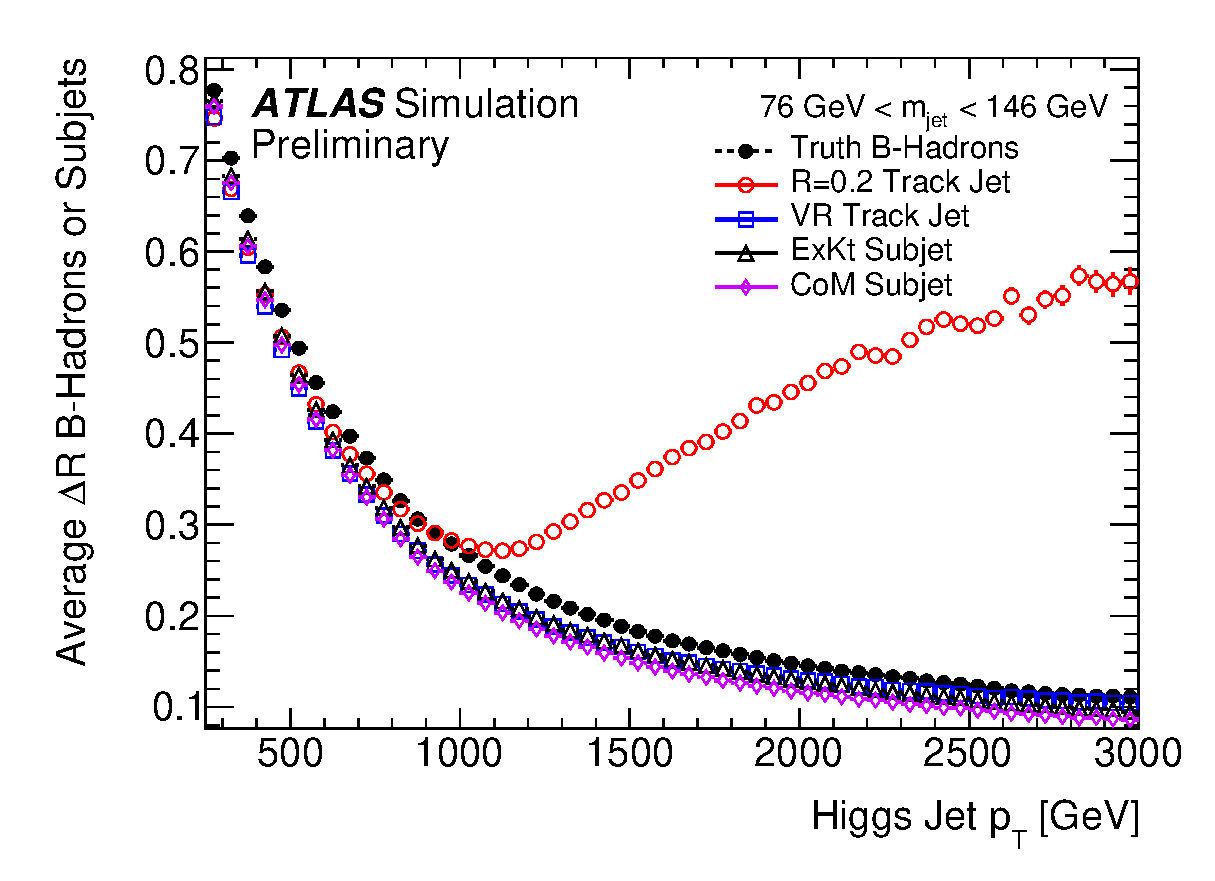
\includegraphics[width=0.8\linewidth]{event_reconstruction/Higgs_VR_DeltaR.eps}
 \caption[The $\Delta R$ between the two leading truth $b$-hadrons or subjets associated to Higgs jets as a function of Higgs jet $p_{T}$.]{%
  The $\Delta R$ between the two leading truth $b$-hadrons or subjets associated to Higgs jets as a function of Higgs jet $p_{T}$~\cite{Salzburger:HammersAndNails}.}
 \label{fig:Higgs_VR_DeltaR}
\end{figure}

\section{Flavor Tagging}\label{section:flavor_tagging}

\TODO{Add flavor tagging complimentary to $b$-jet triggers.}

\section{Taus}\label{section:taus}

Tau leptons also produced in collisions in ATLAS, however, given their short lifetime they will decay into other SM particles before entering the detector subsystems and are reconstructed as other physics objects.
When taus decay they decay to hadrons approximately $64\%$ of the time~\cite{Gallinaro:2014eha}, and to other leptons $36\%$ of the time.
The leptonic decays are reconstructed as muons or electrons, and the hadronic decay modes, usually to pions, they are reconstructed as multi-pronged jets matched with tracks in the ID.
As hadronic decays of the tau also have a displaced secondary vertex they can be a source of fakes for $b$-jets.

\section{Missing Transverse Momentum}\label{section:MET}

Missing transverse momentum, $\MET$ --- or ``MET'' --- is the imbalance of momentum in the transverse plane of the event.
Any event that has neutrinos produced in it, such as events with $W \to \ell \nu_{\ell}$ processes, will have $\MET$ as neutrinos pass through ATLAS without interaction, escaping detection.
However, in events without neutrinos if other physics objects are not properly reconstructed there will still be some $\MET$ in the event.

In closing, given the fully hadronic signature of the analysis signature in the high momentum regime, that will be described in \Cref{chapter:analysis}, and the use of $b$-tagging it is seen that the proper reconstruction of \largeR{} jets with $b$-tagged VR subjets is going to be of great importance.
Additionally, well reconstructed muons will play an important role in the establishment of a $t\bar{t}$ control region.
